\documentclass[12pt]{article}

\usepackage{amsmath}
\usepackage{graphicx}
\usepackage{subfigure}
\usepackage{float}
\usepackage{ulem}
\usepackage{bm}
\usepackage{anysize}

\marginsize{2cm}{2cm}{0.9cm}{1.8cm}

\title{EECE 5639 Computer Vision\\ [2ex] \begin{large} Homework \#2 \end{large} }
\author{Jiyu Tian}
\date{}

\begin{document}
\maketitle
%%---------------------------------------------------------------
%% Question 1
%%---------------------------------------------------------------
\section{Solution:}
As shown in Figure \ref{raw}, the estimated noise of generated images is 1.9462, which is very approximate to 2, the targeted $\sigma$. And the worst case acquisition noise is 4.0258, around $2\sigma$.
\begin{figure}[H]
\centering
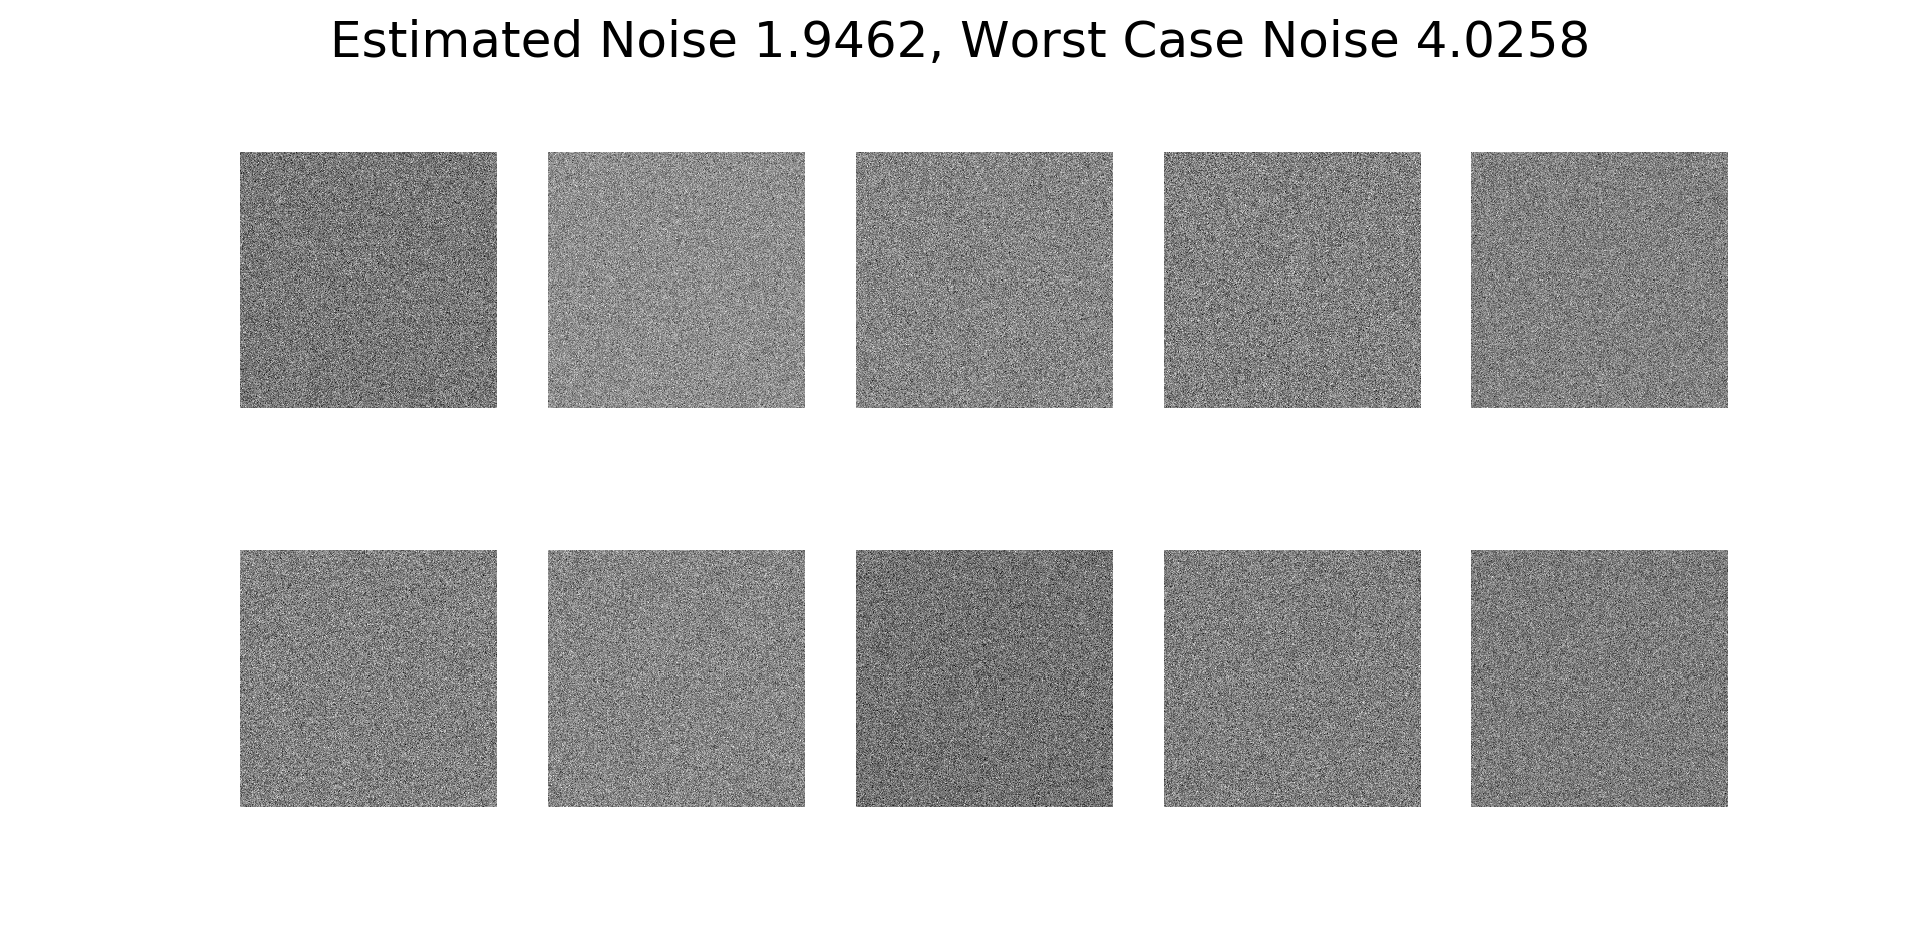
\includegraphics[width = 1\textwidth]{fig1.png}
\caption{Raw Images}
\label{raw}
\end{figure}
%%---------------------------------------------------------------
%% Question 2
%%---------------------------------------------------------------
\section{Solution:}
As shown in Figure \ref{filtered}, the estimated noise of the images after $3\times3$ box filter is 0.6472, and the worst case acquisition noise is 1.3971. Compared to the original ones, the image noises are reduced significantly, which we can also easily tell from the two figures.
\begin{figure}[H]
\centering
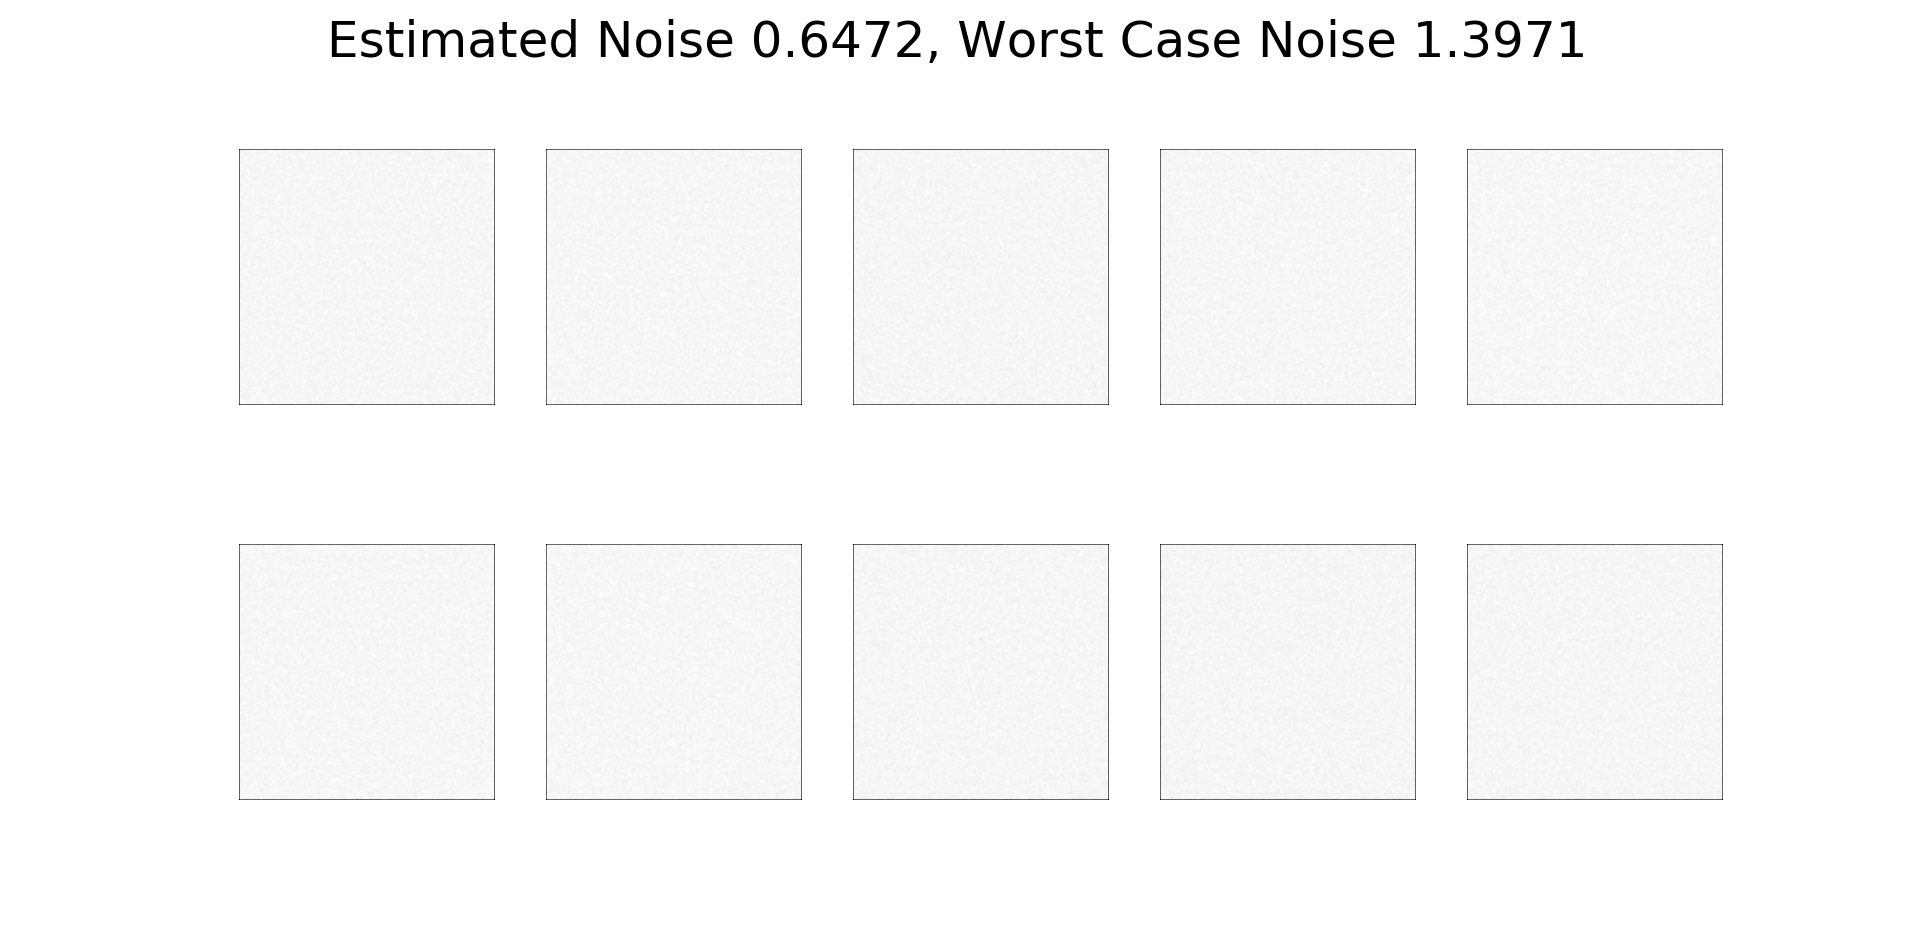
\includegraphics[width = 1\textwidth]{fig2.png}
\caption{Raw Images}
\label{filtered}
\end{figure}
%%---------------------------------------------------------------
%% Question 3
%%---------------------------------------------------------------
\section{Solution:}
\vfill
\clearpage
%%---------------------------------------------------------------
%% Question 4
%%---------------------------------------------------------------
\section{Solution:}
(a) With filter (a): 
\begin{equation*}
{\left[ \begin{array}{cccccccccc}
6 & 8 & 10 & 16 & 22 & 28 & 34&  40 &  32& 24
\end{array} \right]}
\end{equation*}
\noindent With filter (b):
\begin{equation*}
{\left[ \begin{array}{cccccccccc}
7 & 9 & 10 & 13 & 19 & 31 & 37 & 40 & 36 & 28
\end{array} \right]}
\end{equation*}
\noindent (b) Consider a 1D image which is large enough to ignore the borders, with additive, uncorrelated Gaussian noise with zero mean and variance $\sigma^2$. Since filter (b) has different weights upon each filtered pixel, its computation cost is higher than that of filter (a). As for the variance of the noise, with filter (a), a pixel in the output noise $O$ with respect to input noise $I$ is:
\begin{equation*}
O_i = \frac{1}{5}\sum^2_{j = -2}I_{i+j}
\end{equation*}
The expected value of a pixel after filtering is:
\begin{equation*}
E[O] = E\left[\frac{1}{5}\sum^2_{j = -2}I_{i+j}\right] = \frac{1}{5}\sum^2_{j=-2}E\left[I_{i+j}\right] = 0
\end{equation*}
The variance of a pixel after filtering is:
\begin{equation*}
\begin{aligned}
E[(O-E[O])^2] &= E[O^2] \\
&= E\left[\frac{1}{25}\left(\sum^2_{j = -2}I_{i+j}\right)^2\right]\\
&= \frac{1}{25}E\left[\sum^2_{j-2}I^2_{i+j} + \sum^2_{m,n = -2}I_{i+m}I_{i+n}\right]\\
&= \frac{1}{25}\sum^2_{j-2}E\left[I^2_{i+j}\right]\\
&=\frac{1}{25}\times5\sigma^2 = \frac{\sigma^2}{5}
\end{aligned}
\end{equation*}
With filter (b):
\begin{equation*}
O_i = \frac{1}{10}\left(I_{i-2} + 2I_{i-1} + 4I_{i} + 2I_{i+1} + I_{i+2}\right)
\end{equation*}
The expected value of a pixel after filtering is:
\begin{equation*}
\begin{aligned}
E[O] &= E\left(\frac{1}{10}\left[I_{i-2} + 2I_{i-1} + 4I_{i} + 2I_{i+1} + I_{i+2}\right]\right)\\
&= \frac{1}{10}\left[E[I_{i-2}] + E[2I_{i-1}] + E[4I_{i}] + E[2I_{i+1}] + E[I_{i+2}] \right] \\
&= 0
\end{aligned}
\end{equation*}
The variance of a pixel after filtering is:
\begin{equation*}
\begin{aligned}
E[(O-E[O])^2] &= E[O^2] \\
&=\frac{1}{100}E\left[ I^2_{i-2} + 4I^2_{i-1} + 16I^2_{i} + 4I^2_{i+1} + I^2_{i+2} +\sum_l\sum^2_{m,n = -2}\alpha_lI_{i+m}I_{i+n} \right]\\
&=\frac{1}{100}\left[ E[I^2_{i-2}] + 4E[I^2_{i-1}] + 16E[I^2_{i}] + 4E[I^2_{i+1}] + E[I^2_{i+2}] \right]\\
&=\frac{1}{100}\times26\sigma^2=\frac{13}{50}\sigma^2> \frac{\sigma^2}{5}
\end{aligned}
\end{equation*}
Therefore, after these two average filters, the expected value keeps the same. But the variance after filter (b) is larger than that of filter (a).
%%---------------------------------------------------------------
%% Question 5
%%---------------------------------------------------------------
\section{Solution:}



\vfill
\clearpage
%%---------------------------------------------------------------
%% Question 6
%%---------------------------------------------------------------
\section{Solution:}
The image I is:
\begin{equation*}
I={\left[ \begin{array}{cccccccc}
0 & 1 & 2 & 3 & 4 & 5 & 6 & 7\\
1 & 0 & 1 & 2 & 3 & 4 & 5 & 6\\
2 & 1 & 0 & 1 & 2 & 3 & 4 & 5\\
3 & 2 & 1 & 0 & 1 & 2 & 3 & 4\\
4 & 3 & 2 & 1 & 0 & 1 & 2 & 3\\
5 & 4 & 3 & 2 & 1 & 0 & 1 & 2\\
6 & 5 & 4 & 3 & 2 & 1 & 0 & 1\\
7 & 6 & 5 & 4 & 3 & 2 & 1 & 0\\
\end{array} \right]}
\end{equation*}
After applying a $3\times3$ median filter, the output is 
\begin{equation*}
O={\left[ \begin{array}{cccccccc}
0 & 1 & 2 & 3 & 4 & 5 & 6 & 7\\
1 & 1 & 1 & 2 & 3 & 4 & 5 & 6\\
2 & 1 & 1 & 1 & 2 & 3 & 4 & 5\\
3 & 2 & 1 & 1 & 1 & 2 & 3 & 4\\
4 & 3 & 2 & 1 & 1 & 1 & 2 & 3\\
5 & 4 & 3 & 2 & 1 & 1 & 1 & 2\\
6 & 5 & 4 & 3 & 2 & 1 & 1 & 1\\
7 & 6 & 5 & 4 & 3 & 2 & 1 & 0\\
\end{array} \right]}
\end{equation*}

%%---------------------------------------------------------------
%% Question 7
%%---------------------------------------------------------------
\section{Solution:}
The input image is:
\begin{equation*}
I={\left[ \begin{array}{cccccccc}
4 & 4 & 4 & 4 & 8 & 8 & 8 & 8
\end{array} \right]}
\end{equation*}
After applying the median filter assuming that the border pixels are not changed:
\begin{equation*}
I={\left[ \begin{array}{cccccccc}
4 & 4 & 4 & 4 & 8 & 8 & 8 & 8
\end{array} \right]}
\end{equation*}
After applying the averaging mask assuming that the border pixels are not changed:
\begin{equation*}
I={\left[ \begin{array}{cccccccc}
4 & 4 & 4 & 5 & 7 & 8 & 8 & 8
\end{array} \right]}
\end{equation*}
The median filter keeps the step image unchanged, while the averaging mask smooths the step.
 
\end{document}
